\chapter{EXPERIMENTS WITH MULTIPLE DESIGN FACTORS}
\makeheading{Week 7}
\begin{itemize}
      \item We now consider the design and analysis of experiments consisting of multiple conditions arising
            from multiple design factors.
            \begin{itemize}
                  \item This is often colloquially referred to as ``multivariate testing'' (MVT).
            \end{itemize}
      \item Canonical MVT button test:
            \begin{figure}[!htbp]
                  \centering
                  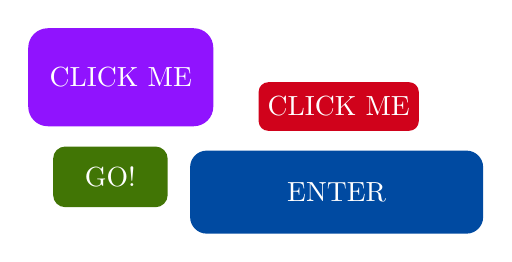
\begin{tikzpicture}[x=0.75pt,y=0.75pt,yscale=-1,xscale=1]
                        %uncomment if require: \path (0,105); %set diagram left start at 0, and has height of 105

                        %Rounded Rect [id:dp8976617722511913] 
                        \draw  [draw opacity=0][fill={rgb, 255:red, 208; green, 2; blue, 27 }  ,fill opacity=1 ] (112,31.79) .. controls (112,29.2) and (114.1,27.1) .. (116.69,27.1) -- (184.48,27.1) .. controls (187.07,27.1) and (189.17,29.2) .. (189.17,31.79) -- (189.17,45.85) .. controls (189.17,48.44) and (187.07,50.53) .. (184.48,50.53) -- (116.69,50.53) .. controls (114.1,50.53) and (112,48.44) .. (112,45.85) -- cycle ;
                        %Rounded Rect [id:dp05576705853009267] 
                        \draw  [draw opacity=0][fill={rgb, 255:red, 0; green, 74; blue, 161 }  ,fill opacity=1 ] (79,68.07) .. controls (79,63.65) and (82.58,60.07) .. (87,60.07) -- (212.17,60.07) .. controls (216.58,60.07) and (220.17,63.65) .. (220.17,68.07) -- (220.17,92.07) .. controls (220.17,96.48) and (216.58,100.07) .. (212.17,100.07) -- (87,100.07) .. controls (82.58,100.07) and (79,96.48) .. (79,92.07) -- cycle ;
                        %Rounded Rect [id:dp1316893319581255] 
                        \draw  [draw opacity=0][fill={rgb, 255:red, 65; green, 117; blue, 5 }  ,fill opacity=1 ] (13,63.95) .. controls (13,60.72) and (15.62,58.1) .. (18.85,58.1) -- (62.32,58.1) .. controls (65.55,58.1) and (68.17,60.72) .. (68.17,63.95) -- (68.17,81.49) .. controls (68.17,84.72) and (65.55,87.33) .. (62.32,87.33) -- (18.85,87.33) .. controls (15.62,87.33) and (13,84.72) .. (13,81.49) -- cycle ;
                        %Rounded Rect [id:dp1823408740718886] 
                        \draw  [draw opacity=0][fill={rgb, 255:red, 144; green, 19; blue, 254 }  ,fill opacity=1 ] (1,10.55) .. controls (1,5.33) and (5.23,1.1) .. (10.45,1.1) -- (80.72,1.1) .. controls (85.94,1.1) and (90.17,5.33) .. (90.17,10.55) -- (90.17,38.89) .. controls (90.17,44.1) and (85.94,48.33) .. (80.72,48.33) -- (10.45,48.33) .. controls (5.23,48.33) and (1,44.1) .. (1,38.89) -- cycle ;

                        % Text Node
                        \draw (150.58,38.82) node  [color={rgb, 255:red, 255; green, 255; blue, 255 }  ,opacity=1 ] [align=left] {CLICK ME};
                        % Text Node
                        \draw (149.58,80.07) node  [color={rgb, 255:red, 255; green, 255; blue, 255 }  ,opacity=1 ] [align=left] {ENTER};
                        % Text Node
                        \draw (40.58,72.72) node  [color={rgb, 255:red, 255; green, 255; blue, 255 }  ,opacity=1 ] [align=left] {GO!};
                        % Text Node
                        \draw (45.58,24.72) node  [color={rgb, 255:red, 255; green, 255; blue, 255 }  ,opacity=1 ] [align=left] {CLICK ME};
                  \end{tikzpicture}
            \end{figure}

            Many things influence click-through rate:
            \begin{itemize}
                  \item Colour.
                  \item Size.
                  \item Position.
                  \item Phrase.
            \end{itemize}
      \item Some additional, more tangible, examples:
            \begin{itemize}
                  \item \href{https://goodui.org/leaks/how-etsys-product-page-design-evolved-between-2019-and-2020/}{Etsy}.
                  \item \href{https://goodui.org/leaks/netflix-a-b-tests-4-secondary-choices-all-of-which-get-rejected/}{Netflix}.
                  \item \href{https://goodui.org/leaks/airbnb-a-b-tests-and-rejects-a-natural-language-form/}{Airbnb}.
            \end{itemize}
      \item This week we describe how to design and analyze experiments that efficiently investigate multiple
            design factors.
      \item \textbf{Goals}:
            \begin{enumerate}[1.]
                  \item Determine which condition is optimal with respect to some metric of interest.
                        \begin{itemize}
                              \item But now a condition is defined by a specific combination of the levels of \emph{multiple} design factors.
                        \end{itemize}
                  \item Determine \emph{which} factors are influential and understand \emph{how} the factors influence the response.
            \end{enumerate}
\end{itemize}
\section{The Factorial Approach}
\begin{itemize}
      \item The key to multi-factor experiments is to \emph{efficiently} investigate different combinations of the factor
            levels.
      \item \textbf{One-factor-at-a-time approach} (OFAT):
            \begin{itemize}
                  \item Sequence of experiments, each with just one factor being varied.
                  \item The winning level of this factor is retained.
                  \item Follow-up experiments manipulate some other factor, while the previous ones are held fixed at
                        their optimal levels.
                        \begin{Example}{Button}{}
                              \begin{enumerate}[1.]
                                    \item Experiment with colour, and purple wins.
                                    \item Experiment with phrase, and ``submit'' wins.
                                    \item Experiment with size, and ``large'' wins.
                              \end{enumerate}
                        \end{Example}
            \end{itemize}
\end{itemize}
\begin{Example}{Twitter $ \heartsuit $ versus $ \star $}{twit_ex}
      \begin{itemize}
            \item In 2015 Twitter changed ``favouriting'' a tweet (expressed as stars) to ``liking'' a tweet (expressed
                  as hearts) and \href{https://entertainment.ie/trending/twitter-changed-their-star-favourites-to-heart-likes-and-the-internet-is-pissed-335920/}{the internet was pissed}.
            \item In line with Twitter's ``test everything'' motto, this decision came about as a result of experimentation.
            \item A hypothetical experiment that could have lead to this decision might involve two factors at two levels.
                  \begin{itemize}
                        \item $ \text{DF1}=\text{Shape}\to\Set{\text{Star},\text{Heart}} $.
                        \item $ \text{DF2}=\text{Colour}\to\Set{\text{Yellow},\text{Red}} $.
                  \end{itemize}
            \item A one-factor-at-a-time approach might look like this:
                  \begin{itemize}
                        \item Experiment 1: $ \color{Gold}\star $ versus $ \color{Gold}\heartsuit $.
                        \item Experiment 2: $ \color{Gold}\star $ versus $ \color{Red}\heartsuit $.
                  \end{itemize}
            \item Suppose they conclude that $ \color{Red}\heartsuit $ is the best, but what about $ \color{Red}\star $?
                  The problem with OFAT experiments is that we may never observe the truly optimal combination of factor levels.
      \end{itemize}
\end{Example}
\begin{Example}{Etsy Search Bar}{}
      \begin{itemize}
            \item \href{https://goodui.org/leaks/how-etsys-product-page-design-evolved-between-2019-and-2020/}{Check it out}.
      \end{itemize}
\end{Example}
\begin{itemize}
      \item \textbf{The Factorial approach}:
            \begin{itemize}
                  \item Experimental conditions are defined as every unique combination of the design factors' levels.
                  \item In the \textbf{Twitter} example, the factorial experiment would have looked like this:
                        $ \color{Gold}\star\color{Red}\star\color{Gold}\heartsuit\color{Red}\heartsuit $.
                  \item In the \textbf{Etsy} example, the factorial experiment would have looked like this:
                        \begin{tightcenter}
                              \emph{Small Square Box}, \emph{Small Rounded Box}, \emph{Long Square Box}, \emph{Long Rounded Box}.
                        \end{tightcenter}
                  \item \textbf{Advantage}: it explores every possible condition.
                        \begin{enumerate}[1.]
                              \item We don't miss the optimal condition.
                              \item Our understanding of the relationship between the response and design factors is better with a factorial experiment than with an OFAT experiment.
                        \end{enumerate}
                  \item \textbf{Disadvantage}: it explores every possible condition.
                        \begin{itemize}
                              \item With many design factors at many levels, the number of unique combinations might be unmanageably large.
                        \end{itemize}
                  \item As long as we choose our factors and their levels thoughtfully, the advantages outweigh the
                        disadvantages.
            \end{itemize}
      \item \textbf{Main effects}: The main effect of factor A, represents the change in the response variable produced
            by a change in that factor. In our \hyperref[ex:twit_ex]{\textbf{Twitter}} example:
            \begin{itemize}
                  \item Main effect of shape: what happens to the response when we change the shape from $ \star $ to $ \heartsuit $.
                  \item Main effect of colour: what happens to the response when we change the colour from yellow to red?
            \end{itemize}
      \item \textbf{Interaction effects}: If the main effect of factor A depends on the level of some other factor B, we
            say that factors A and B interact. In our \hyperref[ex:twit_ex]{\textbf{Twitter}} example:
            \begin{itemize}
                  \item Is there an interaction between shape and colour?
                        \begin{itemize}[$\iff$]
                              \item Does the effect of going from $ \star $ to $ \heartsuit $ depend on colour?
                              \item Does the effect of going from yellow to red depend on shape?
                        \end{itemize}
            \end{itemize}
      \item From a practical perspective it is critical to quantify both types of effects.
            \begin{itemize}
                  \item The only type of design that allows us to observe and estimate both main and interaction effects
                        is the factorial design. The OFAT cannot do this.
            \end{itemize}
\end{itemize}
\section{Designing a Factorial Experiment}
\begin{itemize}
      \item Conceptually, the design of a factorial experiment is simple.
            \begin{enumerate}[1.]
                  \item Pick your metric of interest and define the corresponding response variable.
                  \item Pick your design factors.
                  \item Pick their levels.
                  \item Define your experimental conditions (all possible combinations of our design factors' levels).
                  \item Determine your sample sizes.
            \end{enumerate}
            \begin{Example}{Button}{}
                  Suppose you have $ K=3 $ factors, \emph{colour} (red, blue), \emph{phrase} (``Continue'', ``Go''),
                  and \emph{size} (small, medium, large). These factors therefore have $ m_1=2 $, $ m_2=2 $, and $ m_3=3 $
                  levels respectively. Therefore, we have $ m=m_1m_2m_3=(2)(2)(3)=12 $ experimental conditions.
                  \begin{center}
                        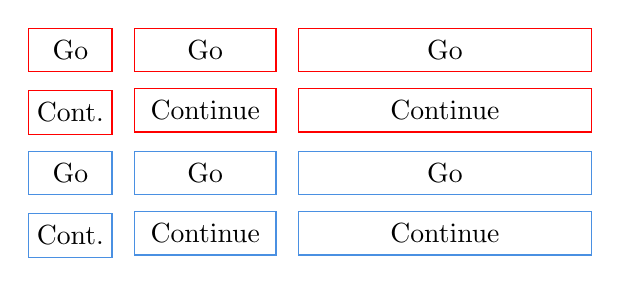
\begin{tikzpicture}[x=0.75pt,y=0.75pt,yscale=-1,xscale=1]
                              %uncomment if require: \path (0,129); %set diagram left start at 0, and has height of 129

                              %Shape: Rectangle [id:dp10311262728916426] 
                              \draw  [color={rgb, 255:red, 255; green, 0; blue, 0 }  ,draw opacity=1 ] (10,10.1) -- (50.17,10.1) -- (50.17,31.1) -- (10,31.1) -- cycle ;
                              %Shape: Rectangle [id:dp4509704567871202] 
                              \draw  [color={rgb, 255:red, 255; green, 0; blue, 0 }  ,draw opacity=1 ] (61,10.1) -- (129.17,10.1) -- (129.17,31.1) -- (61,31.1) -- cycle ;
                              %Shape: Rectangle [id:dp6775011225238754] 
                              \draw  [color={rgb, 255:red, 255; green, 0; blue, 0 }  ,draw opacity=1 ] (140,10.1) -- (281.17,10.1) -- (281.17,31.1) -- (140,31.1) -- cycle ;
                              %Shape: Rectangle [id:dp4806563569724954] 
                              \draw  [color={rgb, 255:red, 255; green, 0; blue, 0 }  ,draw opacity=1 ] (10,40.1) -- (50.17,40.1) -- (50.17,61.1) -- (10,61.1) -- cycle ;
                              %Shape: Rectangle [id:dp8355991781261779] 
                              \draw  [color={rgb, 255:red, 255; green, 0; blue, 0 }  ,draw opacity=1 ] (61,39.1) -- (129.17,39.1) -- (129.17,60.1) -- (61,60.1) -- cycle ;
                              %Shape: Rectangle [id:dp4978491167910569] 
                              \draw  [color={rgb, 255:red, 255; green, 0; blue, 0 }  ,draw opacity=1 ] (140,39.1) -- (281.17,39.1) -- (281.17,60.1) -- (140,60.1) -- cycle ;
                              %Shape: Rectangle [id:dp20386766165344195] 
                              \draw  [color={rgb, 255:red, 74; green, 144; blue, 226 }  ,draw opacity=1 ] (10,69.37) -- (50.17,69.37) -- (50.17,90.37) -- (10,90.37) -- cycle ;
                              %Shape: Rectangle [id:dp6104253470815134] 
                              \draw  [color={rgb, 255:red, 74; green, 144; blue, 226 }  ,draw opacity=1 ] (61,69.37) -- (129.17,69.37) -- (129.17,90.37) -- (61,90.37) -- cycle ;
                              %Shape: Rectangle [id:dp237793543875083] 
                              \draw  [color={rgb, 255:red, 74; green, 144; blue, 226 }  ,draw opacity=1 ] (140,69.37) -- (281.17,69.37) -- (281.17,90.37) -- (140,90.37) -- cycle ;
                              %Shape: Rectangle [id:dp1886700894445873] 
                              \draw  [color={rgb, 255:red, 74; green, 144; blue, 226 }  ,draw opacity=1 ] (10,99.37) -- (50.17,99.37) -- (50.17,120.37) -- (10,120.37) -- cycle ;
                              %Shape: Rectangle [id:dp767578747937531] 
                              \draw  [color={rgb, 255:red, 74; green, 144; blue, 226 }  ,draw opacity=1 ] (61,98.37) -- (129.17,98.37) -- (129.17,119.37) -- (61,119.37) -- cycle ;
                              %Shape: Rectangle [id:dp12570152585404148] 
                              \draw  [color={rgb, 255:red, 74; green, 144; blue, 226 }  ,draw opacity=1 ] (140,98.37) -- (281.17,98.37) -- (281.17,119.37) -- (140,119.37) -- cycle ;

                              % Text Node
                              \draw (30.08,20.6) node   [align=left] {Go};
                              % Text Node
                              \draw (30.08,50.6) node   [align=left] {Cont.};
                              % Text Node
                              \draw (95.08,20.6) node   [align=left] {Go};
                              % Text Node
                              \draw (210.58,20.6) node   [align=left] {Go};
                              % Text Node
                              \draw (95.08,49.6) node   [align=left] {Continue};
                              % Text Node
                              \draw (210.58,49.6) node   [align=left] {Continue};
                              % Text Node
                              \draw (30.08,79.87) node   [align=left] {Go};
                              % Text Node
                              \draw (30.08,109.87) node   [align=left] {Cont.};
                              % Text Node
                              \draw (95.08,79.87) node   [align=left] {Go};
                              % Text Node
                              \draw (210.58,79.87) node   [align=left] {Go};
                              % Text Node
                              \draw (95.08,108.87) node   [align=left] {Continue};
                              % Text Node
                              \draw (210.58,108.87) node   [align=left] {Continue};
                        \end{tikzpicture}
                  \end{center}
            \end{Example}
      \item In general, a factorial experiment with $K$ factors requires $ m=m_1m_2\cdots m_K $ conditions, where $m_k$ is
            the number of levels of design factor $ k $.
      \item As the number of factors and levels increase, the size of the experiment can get unmanageably large.
            \begin{itemize}
                  \item As such, we want to pick our factors and levels thoughtfully. Keep it simple.
                        \begin{enumerate}[1.]
                              \item Don't investigate factors that are highly correlated.
                              \item Don't choose levels that are very similar.
                              \item Don't choose factors that are hard to manipulate outside an experiment.
                        \end{enumerate}
            \end{itemize}
      \item Once the factors, levels, and hence experimental conditions have been established, experimental units
            must be randomized to each of the $m$ conditions.
            \begin{itemize}
                  \item The number of experimental units assigned to each condition $ n_j $, $ j=1,2,\ldots,m $, can
                        be determined by sample size calculations associated with two-sample tests.
                  \item Make sure to account for the multiple comparison problem.
            \end{itemize}
\end{itemize}
\section{Analyzing a Factorial Experiment}
\begin{itemize}
      \item In order to determine which condition is optimal we use pairwise tests.
      \item In order to determine which factors are influential, and to quantify this influence we use regression.
      \item Whether it's a linear or logistic regression, we use a linear predictor which contains the following terms:
            \begin{itemize}
                  \item An intercept.
                  \item Main effect terms. We represent a factor with $ m_k $ levels using $ m_k-1 $ variables.
                  \item $ \text{Two-factor interaction terms}, \text{three-factor interaction terms},\ldots , \text{$ K $-factor interaction terms} $.
                  \item In general, an $ h $-factor interaction is represented by $ h $-way products of the main effect indicators for the factors involved.
            \end{itemize}
\end{itemize}
\begin{Example}{Button}{}
      With $ K=3 $ factors with $ m_1=2 $, $ m_2=2 $, and $ m_3=3 $ levels, the required linear predictor will contain:
      \begin{itemize}
            \item Main effect terms, and
                  \begin{itemize}
                        \item Let $ x_1 $ be an indicator for ``colour.''
                        \item Let $ x_2 $ be an indicator for ``phrase.''
                        \item Let $ x_3 $ and $ x_4 $ be indicators for ``size.''
                  \end{itemize}
            \item Two-factor interaction terms, and pairwise products of indicators for each pair of factors.
            \item Three-factor interaction terms. Three-way products of the indicators for all three factors.
            \item The linear predictor is given by:
                  \begin{multline*}
                        \beta_0+\underbracket{\beta_1x_1+\beta_2x_2+\beta_3x_3+\beta_4x_4}_{\text{main effects}}\\
                        +\underbracket{\beta_5x_1x_2+\beta_6x_1x_3+\beta_7x_1x_4+\beta_8x_2x_3+\beta_9x_2x_4}_{\text{two-factor interactions}}\\
                        +\underbracket{\beta_{10}x_1x_2x_3+\beta_{11}x_1x_2x_4}_{\text{three-factor interactions}}
                  \end{multline*}
            \item Hypotheses concerning the main effects will therefore involve $ \beta_1,\beta_2,\beta_3,\beta_4 $.
            \item Hypotheses concerning the two-factor interactions will involve $ \beta_5,\beta_6,\beta_7,\beta_8,\beta_9 $.
            \item Hypotheses concerning the three-factor interactions will involve $ \beta_{10},\beta_{11} $.
      \end{itemize}
\end{Example}
\begin{itemize}
      \item In general, hypotheses of these sort will be performed by comparing full versus reduced models via
            partial $F$-tests (in the case of linear regression) and likelihood ratio tests (in the case of logistic
            regression).
\end{itemize}
\subsection{Continuous Response --- The Instagram Example}
\begin{itemize}
      \item We illustrate the topics discussed in this section in the context of an \textbf{Instagram Ad} example.
      \item Suppose that you are a data scientist at Instagram, and you are interested in running an experiment
            to learn about how ad frequency and ad type influences user engagement.
      \item Suppose that ad frequency has levels $ \Set{\text{9:1},\text{7:1},\text{4:1},\text{1:1}} $ corresponding to ad frequencies of
            1 in 10, 1 in 8, 1 in 5, and every other.
      \item Suppose also that ad type is a second design factor with levels $ \Set{\text{photo},\text{video}} $.
      \item We will consider here the factorial experiment that considers every combination of these two factors'
            levels. Therefore, $ m=m_1m_2=(4)(2)=8 $ conditions.
      \item Assume $ n=1000 $ users are randomly assigned to each of these $ m=8 $ conditions, and on each user we measure
            the length of time they engage with the app (in minutes).
      \item We use the resulting data to create the following \textbf{main effect plots} (i.e., the plots of MOI versus
            the levels of each factor) in~\Cref{wk7eff}.
            \begin{figure}[!htbp]
                  \centering
                  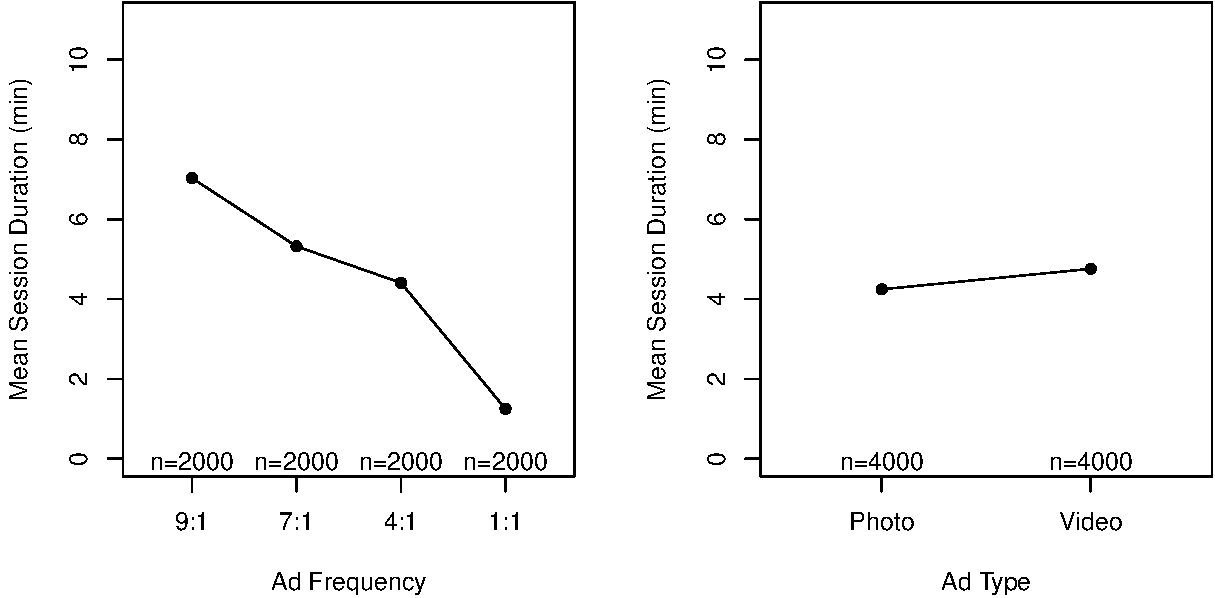
\includegraphics[width=0.8\textwidth]{wk7maineffects.pdf}
                  \caption{Left: Main Effect Plot for Ad Frequency; Right: Main Effect Plot for Ad Type}\label{wk7eff}
            \end{figure}
            \begin{itemize}
                  \item As ad frequency increases, we see that average session duration increases.
                  \item Average session duration increases with video ads relative to photo ads.
                  \item Ad frequency appears to be more influential than ad type since the change in ASD produced by changes in frequency
                        is large (in magnitude) than those produced by changes in ad type.
            \end{itemize}
      \item \textbf{Important}:
            \begin{itemize}
                  \item Discussing main effects can be uninformative and potentially misleading if there is a significant
                        interaction between the factors
                  \item In the presence of a significant interaction effect, it no longer makes sense to discuss the main
                        effect of a factor in isolation, because doing so ignores the fact that this effect changes depending
                        on the level of another factor.
            \end{itemize}
      \item We can evaluate the presence of such interaction by studying \textbf{interaction effect plots} (i.e., plots of the MOI at each
            level of DF1 with different line types distinguishing the levels of DF2) in~\Cref{wk7int}.
            \begin{figure}[!htbp]
                  \centering
                  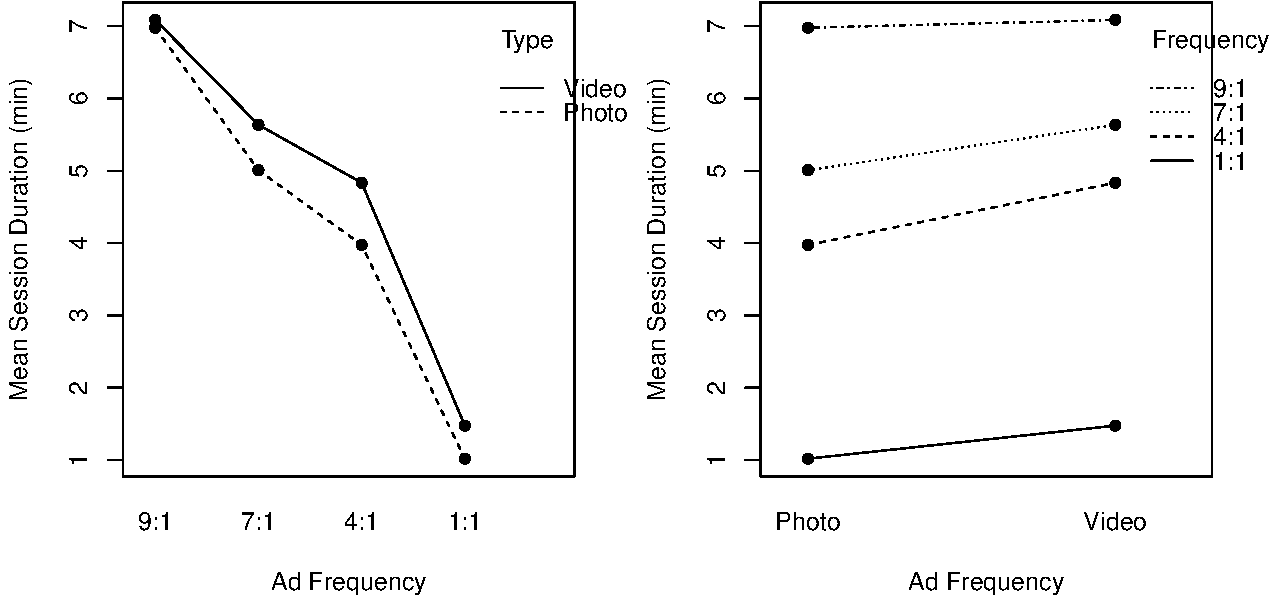
\includegraphics[width=0.8\textwidth]{wk7inteffects.pdf}
                  \caption{Interaction Plot for Ad Frequency and Ad Type.}\label{wk7int}
            \end{figure}
      \item Non-parallel line segments on these plots would indicate the presence of an interaction since this would
            correspond to the main effect of one factor depending on the levels of the other factor.
            \begin{itemize}
                  \item The line segments in these plots are not perfectly parallel and so an interaction appears to exist.
                  \item However, the departure from parallelism is not drastic, and so this interaction is perhaps not strong.
            \end{itemize}
      \item To formally evaluate whether these main effects and interaction effects are significant we fit the following
            linear regression model:
            \[ Y_i=\beta_0+\underbracket{\textcolor{Indigo}{\beta_1x_{i1}+\beta_2x_{i2}+\beta_3x_{i3}}}_{\text{main effects of frequency}}+\underbracket{\textcolor{Fuchsia}{\beta_4x_{i4}}}_{\text{main effects of type}}+
                  \underbracket{\textcolor{Orange}{\beta_5x_{i1}x_{i4}+\beta_6x_{i2}x_{i4}+\beta_7x_{i3}x_{i4}}}_{\text{two-factor interaction}}+\varepsilon_i \]
            where the $ x $'s are indicator variables.
            \begin{itemize}
                  \item $ x_{i1}=1 $ if unit $ i $ is in a condition with the 7:1 ad frequency.
                  \item $ x_{i2}=1 $ if unit $ i $ is in a condition with the 4:1 ad frequency.
                  \item $ x_{i3}=1 $ if unit $ i $ is in a condition with the 1:1 ad frequency.
                  \item $ x_{i4}=1 $ if unit $ i $ is in a condition with video ads.
            \end{itemize}
      \item The expected response in each condition, according to this model is~\Cref{wk7tab1}.
            \begin{table}[!htbp]
                  \centering
                  \begin{NiceTabular}{|cc|c|c|}
                        \toprule            &   & \multicolumn{2}{c} {\emph{Ad Type}}             \\
                        &   & Photo                                          & Video  \\
                        \midrule            & 9:1 & $ \E{Y_i\given x_{i1}=x_{i2}=x_{i3}=0,x_{i4}=0}=\beta_0 $                                          & $ \E{Y_i\given x_{i1}=x_{i2}=x_{i3}=0,x_{i4}=1}=\beta_0+\textcolor{Fuchsia}{\beta_4} $  \\
                        \multirow{2}{*}{\emph{Freq.}} & 7:1 & $ \E{Y_i\given x_{i1}=1,x_{i4}=0}=\beta_0+\beta_1 $                                          & $ \E{Y_i\given x_{i1}=1,x_{i4}=1}=\beta_0+\beta_1+\textcolor{Fuchsia}{\beta_4}+\textcolor{Orange}{\beta_5} $  \\
                        & 4:1 & $ \E{Y_i\given x_{i2}=1,x_{i4}=0}=\beta_0+\beta_2 $                                          & $ \E{Y_i\given x_{i2}=1,x_{i4}=1}=\beta_0+\beta_2+\textcolor{Fuchsia}{\beta_4}+\textcolor{Orange}{\beta_6} $ \\
                        & 1:1 & $ \E{Y_i\given x_{i3}=1,x_{i4}=0}=\beta_0+\beta_3 $                                          & $ \E{Y_i\given x_{i3}=1,x_{i4}=1}=\beta_0+\beta_3+\textcolor{Fuchsia}{\beta_4}+\textcolor{Orange}{\beta_7} $  \\
                        \bottomrule
                  \end{NiceTabular}
                  \caption{Expected Response in Each Ad Frequency-Type Condition}\label{wk7tab1}
            \end{table}
      \item Clearly, a formal test of:
            \begin{tightcenter}
                  \textcolor{Orange}{$ \mathbf{H}_0 $: $ \beta_5=\beta_6=\beta_7=0 $ versus $ \mathbf{H}_\text{A} $: $ \beta_j\ne 0 $}
            \end{tightcenter}
            for $ j=5,6,7 $ would evaluate the significance of the interaction effect.
            \begin{itemize}
                  \item If we reject $ \mathbf{H}_0 $, any conclusions regarding the effect of one factor must be made in the context of
                        the levels of the other factor.
                  \item If we do not reject $ \mathbf{H}_0 $, the interaction terms can be removed from the model yielding the following
                        simplified \textbf{main effects} model:
                        \[ Y_i=\beta_0+\beta_1x_{i1}+\beta_2x_{i2}+\beta_3x_{i3}+\beta_4x_{i4}+\varepsilon_i \]
                        which can be used to evaluate the significance of the main effect of each factor.
                  \item The expected response in each condition, according to the main effects model is~\Cref{wk7tab2}.
                        \begin{table}[!htbp]
                              \centering
                              \begin{NiceTabular}{|cc|c|c|}
                                    \toprule            &   & \multicolumn{2}{c} {\emph{Ad Type}}             \\
                                    &   & Photo                                          & Video  \\
                                    \midrule            & 9:1 & $ \E{Y_i\given x_{i1}=x_{i2}=x_{i3}=0,x_{i4}=0}=\beta_0 $                                          & $ \E{Y_i\given x_{i1}=x_{i2}=x_{i3}=0,x_{i4}=1}=\beta_0+\textcolor{Fuchsia}{\beta_4} $  \\
                                    \multirow{2}{*}{\emph{Freq.}} & 7:1 & $ \E{Y_i\given x_{i1}=1,x_{i4}=0}=\beta_0+\textcolor{Indigo}{\beta_1} $                                          & $ \E{Y_i\given x_{i1}=1,x_{i4}=1}=\beta_0+\textcolor{Indigo}{\beta_1}+\textcolor{Fuchsia}{\beta_4} $  \\
                                    & 4:1 & $ \E{Y_i\given x_{i2}=1,x_{i4}=0}=\beta_0+\textcolor{Indigo}{\beta_2} $                                          & $ \E{Y_i\given x_{i2}=1,x_{i4}=1}=\beta_0+\textcolor{Indigo}{\beta_2}+\textcolor{Fuchsia}{\beta_4} $ \\
                                    & 1:1 & $ \E{Y_i\given x_{i3}=1,x_{i4}=0}=\beta_0+\textcolor{Indigo}{\beta_3} $                                          & $ \E{Y_i\given x_{i3}=1,x_{i4}=1}=\beta_0+\textcolor{Indigo}{\beta_3}+\textcolor{Fuchsia}{\beta_4} $  \\
                                    \bottomrule
                              \end{NiceTabular}
                              \caption{Expected Response in Each Ad Frequency-Type Condition, Based on the Main Effects Model}\label{wk7tab2}
                        \end{table}
                  \item The hypothesis:
                        \begin{tightcenter}
                              \textcolor{Indigo}{$ \mathbf{H}_0 $: $ \beta_1=\beta_2=\beta_3=0 $ versus $ \mathbf{H}_\text{A} $: $ \beta_j\ne 0 $}
                        \end{tightcenter}
                        for $ j=1,2,3 $ tests whether ad frequency is a significant factor.
                  \item The hypothesis:
                        \begin{tightcenter}
                              \textcolor{Fuchsia}{$ \mathbf{H}_0 $: $ \beta_4=0 $ versus $ \mathbf{H}_\text{A} $: $ \beta_4\ne 0 $}
                        \end{tightcenter}
                        tests whether ad type is a significant factor.
                  \item \textbf{But remember}: these tests and the interpretation of main effects are only appropriate in the
                        absence of interaction.
            \end{itemize}
      \item Each of these null hypotheses generates a \textbf{reduced model} with fewer terms relative to a \textbf{full model}
            with all terms --- we compare them using partial $F$-tests associated with an analysis of variance.
      \item Output from the relevant partial F-tests is shown in~\Cref{wk7anova}.
            \begin{figure}[!htbp]
                  \centering
                  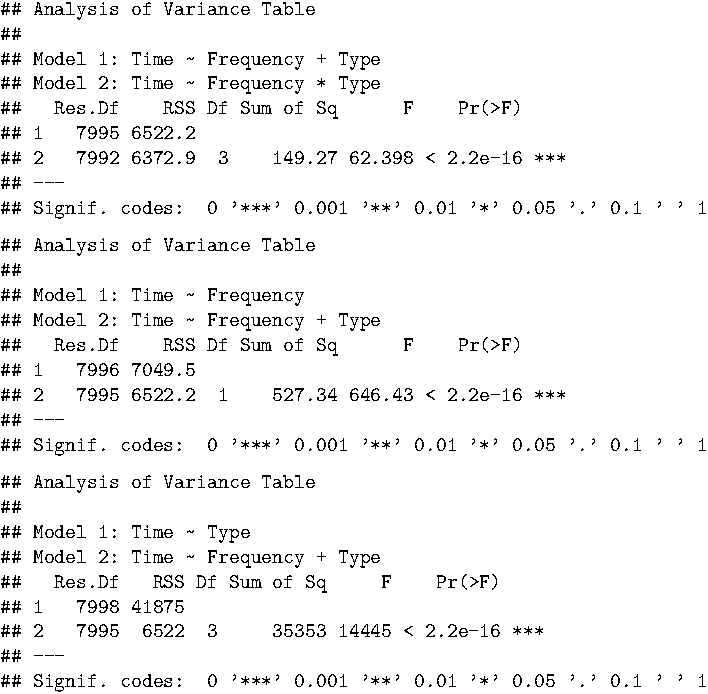
\includegraphics[width=0.8\textwidth]{wk7anova.pdf}
                  \caption{ANOVA Output For Instagram Example}\label{wk7anova}
            \end{figure}
      \item Conclusions:
            \begin{itemize}
                  \item \textcolor{Orange}{The $ p $-value associated with $ \mathbf{H}_0 $: $ \beta_5=\beta_6=\beta_7=0 $ is \underline{very} small, suggesting that the interaction
                              between ad frequency and ad type is significant.}
                  \item \textcolor{Fuchsia}{The $ p $-value associated with $ \mathbf{H}_0 $: $ \beta_4=0 $ is \underline{very} small, suggesting that the main effect of ad type is significant.}
                  \item \textcolor{Indigo}{The $ p $-value associated with $ \mathbf{H}_0 $: $ \beta_1=\beta_2=\beta_3=0 $ is \underline{very} small, suggesting that the main effect of ad frequency is significant.}
                        \begin{itemize}
                              \item Strictly speaking, the last two conclusions are irrelevant because we know the interaction is significant. Although, I include this for \underline{instructional purposes}.
                        \end{itemize}
            \end{itemize}
      \item \href{https://github.com/Hextical/university-notes/blob/master/year-3/semester-3/STAT 430/code/W7/Factorial_example_means.R}{[R Code] \texttt{Factorial\_example\_means}}
\end{itemize}
\subsection{Binary Response --- The TinyCo Example}
\begin{itemize}
      \item The informal and formal evaluation of main and interaction effects can be performed in the context of
            a binary response variable as well.
            \begin{itemize}
                  \item Main effect and interaction effect plots are based on observed proportions.
                  \item Logistic regression is used instead of ordinary linear regression.
            \end{itemize}
      \item The structure of the linear predictor is identical to what we have discussed in general.
      \item For instance, if the Instagram experiment from the previous section had a binary response instead, the
            relevant logistic regression model would be
            \[ \log*{\frac{\pi_i}{1-\pi_i}}=\beta_0+\beta_1x_{i1}+\beta_2x_{i2}+\beta_3x_{i3}+\beta_4x_{i4}+\beta_5x_{i1}x_{i4}+\beta_6x_{i2}x_{i4}+\beta_7x_{i3}x_{i4} \]
            where the $ x $'s are the indicator variables defined previously.
      \item Interest lies in determining whether subsets of the $ \beta $'s are equal to zero to evaluate the significance of
            various main and interaction effects.
            \begin{itemize}
                  \item We use \textbf{likelihood ratio tests} for the comparison of full and reduced logistic regression models.
                  \item The test statistic for the LRT is:
                        \begin{align*}
                              t & =2\log*{\frac{\text{Likelihood}_{\text{Full Model}}}{\text{Likelihood}_{\text{Reduced Model}}}}      \\
                                & =2\Bigl[\text{Log-Likelihood}_{\text{Full Model}}-\text{Log-Likelihood}_{\text{Reduced Model}}\Bigr]
                        \end{align*}
                  \item If $ \mathbf{H}_0 $ is true, then $ t $ should look like it comes from a $ \chi^2(\nu) $ distribution, where
                        \[ \nu=(\#\text{ coefficients in full model})-(\#\text{ coefficients in reduced model}) \]
                  \item $ p\text{-value}=\Prob{T\ge t} $ where $ T \sim \chi^2(\nu) $.
            \end{itemize}
\end{itemize}
